

\tikzset{every picture/.style={line width=1pt}} %set default line width to 0.75pt        

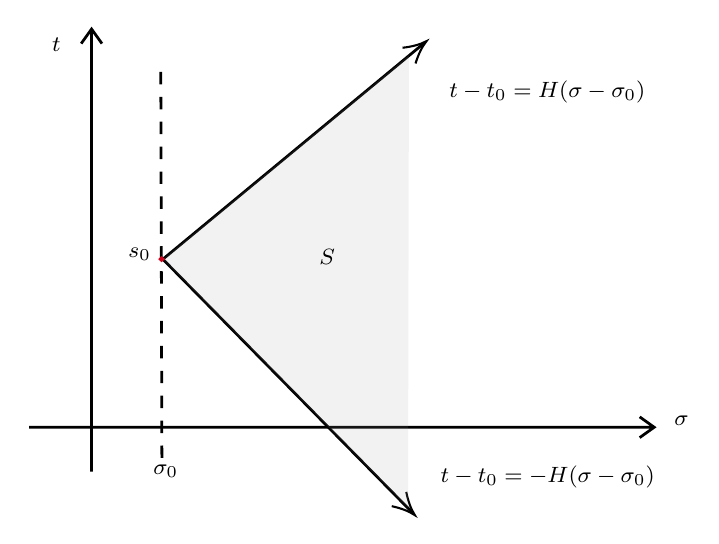
\begin{tikzpicture}[x=0.75pt,y=0.75pt,yscale=-1,xscale=1]
%uncomment if require: \path (0,300); %set diagram left start at 0, and has height of 300

%Shape: Axis 2D [id:dp1346371884561901] 
\draw  (151.5,207.43) -- (452.69,207.43)(181.62,15.58) -- (181.62,228.75) (445.69,202.43) -- (452.69,207.43) -- (445.69,212.43) (176.62,22.58) -- (181.62,15.58) -- (186.62,22.58)  ;
%Straight Lines [id:da6627378326231086] 
\draw  [dash pattern={on 4.5pt off 4.5pt}]  (214.97,36.22) -- (215.5,222.86) ;
%Straight Lines [id:da15935893462766404] 
\draw    (215.34,125.83) -- (336,248.37) ;
\draw [shift={(337.4,249.8)}, rotate = 225.45] [color={rgb, 255:red, 0; green, 0; blue, 0 }  ][line width=0.75]    (10.93,-4.9) .. controls (6.95,-2.3) and (3.31,-0.67) .. (0,0) .. controls (3.31,0.67) and (6.95,2.3) .. (10.93,4.9)   ;
%Straight Lines [id:da1539498165538844] 
\draw    (216,126.43) -- (341.46,22.67) ;
\draw [shift={(343,21.4)}, rotate = 140.41] [color={rgb, 255:red, 0; green, 0; blue, 0 }  ][line width=0.75]    (10.93,-4.9) .. controls (6.95,-2.3) and (3.31,-0.67) .. (0,0) .. controls (3.31,0.67) and (6.95,2.3) .. (10.93,4.9)   ;
%Shape: Ellipse [id:dp5156478132048201] 
\draw  [color={rgb, 255:red, 208; green, 2; blue, 27 }  ,draw opacity=1 ][fill={rgb, 255:red, 208; green, 2; blue, 27 }  ,fill opacity=1 ] (214.69,126.43) .. controls (214.69,126.1) and (214.98,125.83) .. (215.34,125.83) .. controls (215.71,125.83) and (216,126.1) .. (216,126.43) .. controls (216,126.76) and (215.71,127.03) .. (215.34,127.03) .. controls (214.98,127.03) and (214.69,126.76) .. (214.69,126.43) -- cycle ;
%Shape: Right Triangle [id:dp5295703844975419] 
\draw  [draw opacity=0][fill={rgb, 255:red, 155; green, 155; blue, 155 }  ,fill opacity=0.13 ] (334.53,28.25) -- (334.07,246.3) -- (216.03,126.43) -- cycle ;

% Text Node
\draw (160.98,17.94) node [anchor=north west][inner sep=0.75pt]  [font=\footnotesize]  {$t$};
% Text Node
\draw (460.76,200.14) node [anchor=north west][inner sep=0.75pt]  [font=\footnotesize]  {$\sigma $};
% Text Node
\draw (197.73,119.36) node [anchor=north west][inner sep=0.75pt]  [font=\footnotesize]  {$s_{0}$};
% Text Node
\draw (209.68,223.94) node [anchor=north west][inner sep=0.75pt]  [font=\footnotesize]  {$\sigma _{0}$};
% Text Node
\draw (352.39,38.8) node [anchor=north west][inner sep=0.75pt]  [font=\footnotesize]  {$t-t_{0} =H( \sigma -\sigma _{0})$};
% Text Node
\draw (348.09,224.32) node [anchor=north west][inner sep=0.75pt]  [font=\footnotesize]  {$t-t_{0} =-H( \sigma -\sigma _{0})$};
% Text Node
\draw (289.76,120.18) node [anchor=north west][inner sep=0.75pt]  [font=\footnotesize]  {$S$};


\end{tikzpicture}